% Options for packages loaded elsewhere
\PassOptionsToPackage{unicode}{hyperref}
\PassOptionsToPackage{hyphens}{url}
%
\documentclass[
  10.5pt,
]{article}
\title{Econ 144 Project 2}
\author{Shannan Liu, Austin Pham, Zach Wrubel}
\date{13 February, 2022}

\usepackage{amsmath,amssymb}
\usepackage[]{mathpazo}
\usepackage{iftex}
\ifPDFTeX
  \usepackage[T1]{fontenc}
  \usepackage[utf8]{inputenc}
  \usepackage{textcomp} % provide euro and other symbols
\else % if luatex or xetex
  \usepackage{unicode-math}
  \defaultfontfeatures{Scale=MatchLowercase}
  \defaultfontfeatures[\rmfamily]{Ligatures=TeX,Scale=1}
\fi
% Use upquote if available, for straight quotes in verbatim environments
\IfFileExists{upquote.sty}{\usepackage{upquote}}{}
\IfFileExists{microtype.sty}{% use microtype if available
  \usepackage[]{microtype}
  \UseMicrotypeSet[protrusion]{basicmath} % disable protrusion for tt fonts
}{}
\makeatletter
\@ifundefined{KOMAClassName}{% if non-KOMA class
  \IfFileExists{parskip.sty}{%
    \usepackage{parskip}
  }{% else
    \setlength{\parindent}{0pt}
    \setlength{\parskip}{6pt plus 2pt minus 1pt}}
}{% if KOMA class
  \KOMAoptions{parskip=half}}
\makeatother
\usepackage{xcolor}
\IfFileExists{xurl.sty}{\usepackage{xurl}}{} % add URL line breaks if available
\IfFileExists{bookmark.sty}{\usepackage{bookmark}}{\usepackage{hyperref}}
\hypersetup{
  pdftitle={Econ 144 Project 2},
  pdfauthor={Shannan Liu, Austin Pham, Zach Wrubel},
  hidelinks,
  pdfcreator={LaTeX via pandoc}}
\urlstyle{same} % disable monospaced font for URLs
\usepackage[margin=1in]{geometry}
\usepackage{color}
\usepackage{fancyvrb}
\newcommand{\VerbBar}{|}
\newcommand{\VERB}{\Verb[commandchars=\\\{\}]}
\DefineVerbatimEnvironment{Highlighting}{Verbatim}{commandchars=\\\{\}}
% Add ',fontsize=\small' for more characters per line
\usepackage{framed}
\definecolor{shadecolor}{RGB}{248,248,248}
\newenvironment{Shaded}{\begin{snugshade}}{\end{snugshade}}
\newcommand{\AlertTok}[1]{\textcolor[rgb]{0.94,0.16,0.16}{#1}}
\newcommand{\AnnotationTok}[1]{\textcolor[rgb]{0.56,0.35,0.01}{\textbf{\textit{#1}}}}
\newcommand{\AttributeTok}[1]{\textcolor[rgb]{0.77,0.63,0.00}{#1}}
\newcommand{\BaseNTok}[1]{\textcolor[rgb]{0.00,0.00,0.81}{#1}}
\newcommand{\BuiltInTok}[1]{#1}
\newcommand{\CharTok}[1]{\textcolor[rgb]{0.31,0.60,0.02}{#1}}
\newcommand{\CommentTok}[1]{\textcolor[rgb]{0.56,0.35,0.01}{\textit{#1}}}
\newcommand{\CommentVarTok}[1]{\textcolor[rgb]{0.56,0.35,0.01}{\textbf{\textit{#1}}}}
\newcommand{\ConstantTok}[1]{\textcolor[rgb]{0.00,0.00,0.00}{#1}}
\newcommand{\ControlFlowTok}[1]{\textcolor[rgb]{0.13,0.29,0.53}{\textbf{#1}}}
\newcommand{\DataTypeTok}[1]{\textcolor[rgb]{0.13,0.29,0.53}{#1}}
\newcommand{\DecValTok}[1]{\textcolor[rgb]{0.00,0.00,0.81}{#1}}
\newcommand{\DocumentationTok}[1]{\textcolor[rgb]{0.56,0.35,0.01}{\textbf{\textit{#1}}}}
\newcommand{\ErrorTok}[1]{\textcolor[rgb]{0.64,0.00,0.00}{\textbf{#1}}}
\newcommand{\ExtensionTok}[1]{#1}
\newcommand{\FloatTok}[1]{\textcolor[rgb]{0.00,0.00,0.81}{#1}}
\newcommand{\FunctionTok}[1]{\textcolor[rgb]{0.00,0.00,0.00}{#1}}
\newcommand{\ImportTok}[1]{#1}
\newcommand{\InformationTok}[1]{\textcolor[rgb]{0.56,0.35,0.01}{\textbf{\textit{#1}}}}
\newcommand{\KeywordTok}[1]{\textcolor[rgb]{0.13,0.29,0.53}{\textbf{#1}}}
\newcommand{\NormalTok}[1]{#1}
\newcommand{\OperatorTok}[1]{\textcolor[rgb]{0.81,0.36,0.00}{\textbf{#1}}}
\newcommand{\OtherTok}[1]{\textcolor[rgb]{0.56,0.35,0.01}{#1}}
\newcommand{\PreprocessorTok}[1]{\textcolor[rgb]{0.56,0.35,0.01}{\textit{#1}}}
\newcommand{\RegionMarkerTok}[1]{#1}
\newcommand{\SpecialCharTok}[1]{\textcolor[rgb]{0.00,0.00,0.00}{#1}}
\newcommand{\SpecialStringTok}[1]{\textcolor[rgb]{0.31,0.60,0.02}{#1}}
\newcommand{\StringTok}[1]{\textcolor[rgb]{0.31,0.60,0.02}{#1}}
\newcommand{\VariableTok}[1]{\textcolor[rgb]{0.00,0.00,0.00}{#1}}
\newcommand{\VerbatimStringTok}[1]{\textcolor[rgb]{0.31,0.60,0.02}{#1}}
\newcommand{\WarningTok}[1]{\textcolor[rgb]{0.56,0.35,0.01}{\textbf{\textit{#1}}}}
\usepackage{graphicx}
\makeatletter
\def\maxwidth{\ifdim\Gin@nat@width>\linewidth\linewidth\else\Gin@nat@width\fi}
\def\maxheight{\ifdim\Gin@nat@height>\textheight\textheight\else\Gin@nat@height\fi}
\makeatother
% Scale images if necessary, so that they will not overflow the page
% margins by default, and it is still possible to overwrite the defaults
% using explicit options in \includegraphics[width, height, ...]{}
\setkeys{Gin}{width=\maxwidth,height=\maxheight,keepaspectratio}
% Set default figure placement to htbp
\makeatletter
\def\fps@figure{htbp}
\makeatother
\setlength{\emergencystretch}{3em} % prevent overfull lines
\providecommand{\tightlist}{%
  \setlength{\itemsep}{0pt}\setlength{\parskip}{0pt}}
\setcounter{secnumdepth}{-\maxdimen} % remove section numbering
\ifLuaTeX
  \usepackage{selnolig}  % disable illegal ligatures
\fi

\begin{document}
\maketitle

{
\setcounter{tocdepth}{2}
\tableofcontents
}
\newpage

\hypertarget{i.-introduction}{%
\section{I. Introduction}\label{i.-introduction}}

This project contains on 2 components. First, we will fit forecasting
models with a trend, seasonal dummies, and cycles to each of the time
series variables. Then, we will fit VAR models to the data and regress
each series on the other series and itself.

In part 1 of the project, we aim to determine time dependent models that
can capture the stochastic movements of each of the series. In part 2,
we investigate whether or not the addition of other regressors can
improve the forecasting performance of the purely time dependent models.

\hypertarget{brief-background-on-data}{%
\subsection{Brief Background on Data:}\label{brief-background-on-data}}

Sleep Number Corporation (SNBR) is a retail and wholesale company
headquartered in Minneapolis that designs, manufactures, and sells a
line of air bed mattresses. They provide a variety of beds, bedding,
pillows, mattresses, sheets, and duvets for both adults and children.
The company also sells other bedding furniture and accessories, and its
business is focused on consumers in the United States.

Tupperware Brands Corporation (TUP) is consumer discretionary products
company headquartered in Florida. They own a portfolio of global direct
selling companies which sell products across multiple brands and
categories through an independent sales force. The Company's product
brands and categories include food preparation, storage, and serving
solutions for the kitchen and home. Tupperware Brands also sells beauty
and personal care products.

The S\&P 500 Index is a capitalization-weighted index of 505 companies
in the US with the highest market capitalization. It is widely regarded
as the best gauge of large-cap US equities and serves as a benchmark for
many investors. It also includes a wide variety of companies from
different industries and sectors, and it captures 80\% of total market
capitalisation in the US.

SNBR and TUP are related to each other because they are both based in
the US and sell durable consumer goods (although Tupperware Brands also
sells non-durable goods). Therefore, it may be interesting to map our
their relationship through the VAR models. These companies are also
affected by broader US market movements. Hence, we include the S\&P 500
to track that relationship.

\hypertarget{source-of-data}{%
\subsection{Source of Data}\label{source-of-data}}

All of the data was sourced from \url{https://finance.yahoo.com/}. We
will be analyzing weekly observations of the data from December 20, 2010
to February 8, 2022. Company descriptions were adapted from descriptions
provided at \url{https://bloomberg.com}.

\begin{Shaded}
\begin{Highlighting}[]
\CommentTok{\# import data}
\NormalTok{snbr }\OtherTok{=} \FunctionTok{get.hist.quote}\NormalTok{(}\StringTok{"SNBR"}\NormalTok{, }\AttributeTok{start =} \StringTok{"2010{-}12{-}20"}\NormalTok{, }\AttributeTok{end =} \StringTok{"2022{-}02{-}08"}\NormalTok{,}
                     \AttributeTok{quote=}\FunctionTok{c}\NormalTok{(}\StringTok{"Close"}\NormalTok{),}\AttributeTok{provider =} \StringTok{"yahoo"}\NormalTok{,}
                     \AttributeTok{compression =} \StringTok{\textquotesingle{}w\textquotesingle{}}\NormalTok{)}
\end{Highlighting}
\end{Shaded}

\begin{verbatim}
## 'getSymbols' currently uses auto.assign=TRUE by default, but will
## use auto.assign=FALSE in 0.5-0. You will still be able to use
## 'loadSymbols' to automatically load data. getOption("getSymbols.env")
## and getOption("getSymbols.auto.assign") will still be checked for
## alternate defaults.
## 
## This message is shown once per session and may be disabled by setting 
## options("getSymbols.warning4.0"=FALSE). See ?getSymbols for details.
\end{verbatim}

\begin{verbatim}
## time series ends   2022-02-07
\end{verbatim}

\begin{Shaded}
\begin{Highlighting}[]
\NormalTok{tup }\OtherTok{=} \FunctionTok{get.hist.quote}\NormalTok{(}\StringTok{"TUP"}\NormalTok{, }\AttributeTok{start =} \StringTok{"2010{-}12{-}20"}\NormalTok{, }\AttributeTok{end =} \StringTok{"2022{-}02{-}08"}\NormalTok{,}
                       \AttributeTok{quote=}\FunctionTok{c}\NormalTok{(}\StringTok{"Close"}\NormalTok{),}\AttributeTok{provider =} \StringTok{"yahoo"}\NormalTok{,}
                     \AttributeTok{compression =} \StringTok{\textquotesingle{}w\textquotesingle{}}\NormalTok{)}
\end{Highlighting}
\end{Shaded}

\begin{verbatim}
## time series ends   2022-02-07
\end{verbatim}

\begin{Shaded}
\begin{Highlighting}[]
\NormalTok{sp500 }\OtherTok{=} \FunctionTok{get.hist.quote}\NormalTok{(}\StringTok{"\^{}gspc"}\NormalTok{, }\AttributeTok{start =} \StringTok{"2010{-}12{-}20"}\NormalTok{, }\AttributeTok{end =} \StringTok{"2022{-}02{-}08"}\NormalTok{,}
                       \AttributeTok{quote=}\FunctionTok{c}\NormalTok{(}\StringTok{"Close"}\NormalTok{),}\AttributeTok{provider =} \StringTok{"yahoo"}\NormalTok{,}
                     \AttributeTok{compression =} \StringTok{\textquotesingle{}w\textquotesingle{}}\NormalTok{)}
\end{Highlighting}
\end{Shaded}

\begin{verbatim}
## time series ends   2022-02-07
\end{verbatim}

\begin{Shaded}
\begin{Highlighting}[]
\CommentTok{\# there are no NA values }
\FunctionTok{cat}\NormalTok{(}\StringTok{"Number of NA values in SNBR series:"}\NormalTok{,}\FunctionTok{sum}\NormalTok{(}\FunctionTok{is.na}\NormalTok{(snbr)),}\StringTok{"}\SpecialCharTok{\textbackslash{}n}\StringTok{"}\NormalTok{)}
\end{Highlighting}
\end{Shaded}

\begin{verbatim}
## Number of NA values in SNBR series: 0
\end{verbatim}

\begin{Shaded}
\begin{Highlighting}[]
\FunctionTok{cat}\NormalTok{(}\StringTok{"Number of NA values in TUP series:"}\NormalTok{,}\FunctionTok{sum}\NormalTok{(}\FunctionTok{is.na}\NormalTok{(tup)),}\StringTok{"}\SpecialCharTok{\textbackslash{}n}\StringTok{"}\NormalTok{)}
\end{Highlighting}
\end{Shaded}

\begin{verbatim}
## Number of NA values in TUP series: 0
\end{verbatim}

\begin{Shaded}
\begin{Highlighting}[]
\FunctionTok{cat}\NormalTok{(}\StringTok{"Number of NA values in S\&P 500 series:"}\NormalTok{,}\FunctionTok{sum}\NormalTok{(}\FunctionTok{is.na}\NormalTok{(sp500)))}
\end{Highlighting}
\end{Shaded}

\begin{verbatim}
## Number of NA values in S&P 500 series: 0
\end{verbatim}

\begin{Shaded}
\begin{Highlighting}[]
\CommentTok{\# create data frame in case we may need it later}
\NormalTok{df }\OtherTok{=} \FunctionTok{data.frame}\NormalTok{(}\FunctionTok{merge}\NormalTok{(snbr,tup,sp500))}
\NormalTok{df }\OtherTok{\textless{}{-}}\NormalTok{ tibble}\SpecialCharTok{::}\FunctionTok{rownames\_to\_column}\NormalTok{(df,}\StringTok{"dates"}\NormalTok{)}
\NormalTok{df}\SpecialCharTok{$}\NormalTok{dates}\OtherTok{\textless{}{-}}\FunctionTok{as.Date}\NormalTok{(df}\SpecialCharTok{$}\NormalTok{dates,}\StringTok{"\%Y{-}\%m{-}\%d"}\NormalTok{)}

\CommentTok{\# check}
\FunctionTok{head}\NormalTok{(df)}
\end{Highlighting}
\end{Shaded}

\begin{verbatim}
##        dates Close.snbr Close.tup Close.sp500
## 1 2010-12-20       9.25     48.21     1256.77
## 2 2010-12-27       9.13     47.67     1257.64
## 3 2011-01-03      10.46     47.12     1271.50
## 4 2011-01-10      10.37     47.27     1293.24
## 5 2011-01-17      10.26     46.20     1283.35
## 6 2011-01-24      10.03     45.63     1276.34
\end{verbatim}

\newpage

\hypertarget{ii.-results}{%
\section{II. Results}\label{ii.-results}}

\hypertarget{a-produce-a-time-series-plot-of-your-data-including-the-respective-acf-and-pacf-plots.}{%
\subsection{(A) Produce a time-series plot of your data including the
respective ACF and PACF
plots.}\label{a-produce-a-time-series-plot-of-your-data-including-the-respective-acf-and-pacf-plots.}}

\begin{Shaded}
\begin{Highlighting}[]
\FunctionTok{library}\NormalTok{(glue)}
\NormalTok{tsplot }\OtherTok{\textless{}{-}} \ControlFlowTok{function}\NormalTok{(y,series\_name) \{}
  \DocumentationTok{\#\#\#\#\#\#\#\#\#\#\#\#\#\#\#\#\#\#\#\#\#\#\#\#\#\#\#\#\#\#\#\#\#}
  \CommentTok{\# Plot the original time series }
  \CommentTok{\# A histogram of the series     }
  \CommentTok{\# ACF and PACF plots}
  \DocumentationTok{\#\#\#\#\#\#\#\#\#\#\#\#\#\#\#\#\#\#\#\#\#\#\#\#\#\#\#\#\#\#\#\#\#}
\NormalTok{  ax1 }\OtherTok{=} \FunctionTok{autoplot.zoo}\NormalTok{(y, }\AttributeTok{main =} \FunctionTok{sprintf}\NormalTok{(}\StringTok{"\%s Closing Price"}\NormalTok{,series\_name),}
         \AttributeTok{ylab =} \StringTok{"Price (USD)"}\NormalTok{,}\AttributeTok{xlab =} \StringTok{"Time"}\NormalTok{)}
  \StringTok{\textasciigrave{}}\AttributeTok{Closing Price}\StringTok{\textasciigrave{}} \OtherTok{=}\NormalTok{ y}
\NormalTok{  ax2 }\OtherTok{=} \FunctionTok{gghistogram}\NormalTok{(}\StringTok{\textasciigrave{}}\AttributeTok{Closing Price}\StringTok{\textasciigrave{}}\NormalTok{)}
\NormalTok{  ax3 }\OtherTok{=} \FunctionTok{ggAcf}\NormalTok{(y,}
              \AttributeTok{main =} \FunctionTok{glue}\NormalTok{(}\StringTok{\textquotesingle{}\{series\_name\} Sample Autocorrelations\textquotesingle{}}\NormalTok{),}
              \AttributeTok{xlab=}\StringTok{"Displacement"}\NormalTok{,}\AttributeTok{lag.max =} \DecValTok{48}\NormalTok{)}
\NormalTok{  ax4 }\OtherTok{=} \FunctionTok{ggPacf}\NormalTok{(y,}
               \AttributeTok{main =} \FunctionTok{glue}\NormalTok{(}\StringTok{\textquotesingle{}\{series\_name\} Sample Partial Autocorrelations\textquotesingle{}}\NormalTok{),}
               \AttributeTok{xlab=}\StringTok{"Displacement"}\NormalTok{,}\AttributeTok{lag.max =} \DecValTok{48}\NormalTok{)}
  \FunctionTok{grid.arrange}\NormalTok{(ax1, ax2,ax3,ax4, }\AttributeTok{ncol=}\DecValTok{2}\NormalTok{,}\AttributeTok{nrow =} \DecValTok{2}\NormalTok{)}
\NormalTok{\}}

\CommentTok{\# time{-}series, histogram, ACF and PACF plots}
\FunctionTok{tsplot}\NormalTok{(snbr,}\StringTok{"SNBR"}\NormalTok{)}
\end{Highlighting}
\end{Shaded}

\begin{verbatim}
## Warning: Ignoring unknown parameters: main, xlab
## Ignoring unknown parameters: main, xlab
\end{verbatim}

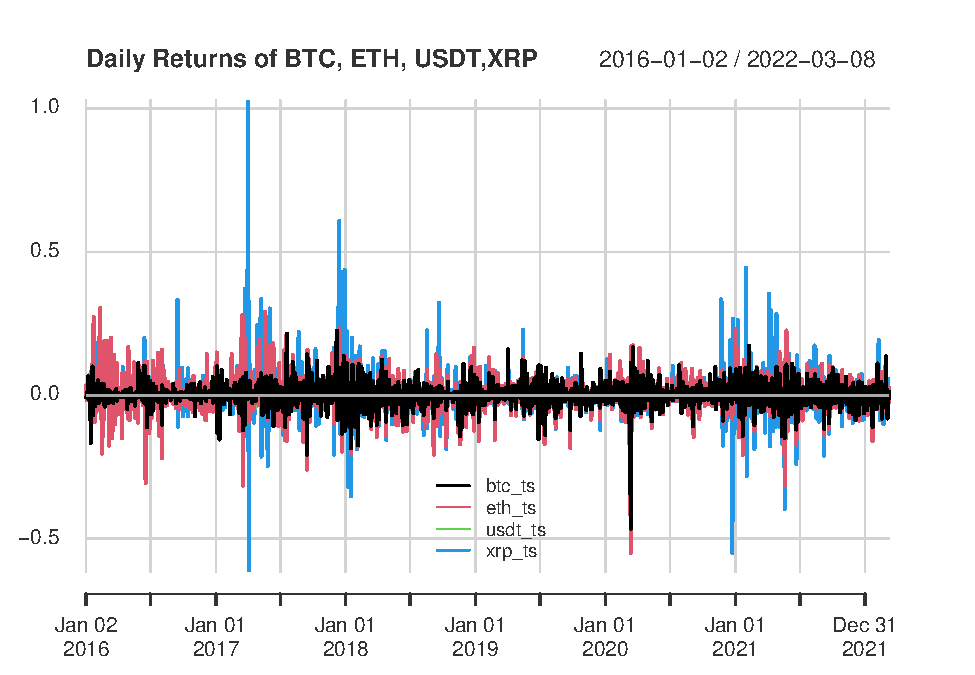
\includegraphics{project2_files/figure-latex/unnamed-chunk-2-1.pdf}

\begin{Shaded}
\begin{Highlighting}[]
\FunctionTok{tsplot}\NormalTok{(tup,}\StringTok{"TUP"}\NormalTok{)}
\end{Highlighting}
\end{Shaded}

\begin{verbatim}
## Warning: Ignoring unknown parameters: main, xlab
## Ignoring unknown parameters: main, xlab
\end{verbatim}

\includegraphics{project2_files/figure-latex/unnamed-chunk-2-2.pdf}

\begin{Shaded}
\begin{Highlighting}[]
\FunctionTok{tsplot}\NormalTok{(sp500,}\StringTok{"S\&P 500"}\NormalTok{)}
\end{Highlighting}
\end{Shaded}

\begin{verbatim}
## Warning: Ignoring unknown parameters: main, xlab
## Ignoring unknown parameters: main, xlab
\end{verbatim}

\includegraphics{project2_files/figure-latex/unnamed-chunk-2-3.pdf}

\hypertarget{b-plot-the-stldecomposition-plot-of-your-data-and-discuss-the-results.}{%
\subsection{(B) Plot the stldecomposition plot of your data, and discuss
the
results.}\label{b-plot-the-stldecomposition-plot-of-your-data-and-discuss-the-results.}}

\begin{Shaded}
\begin{Highlighting}[]
\CommentTok{\# create the time series objects of the closing prices}
\CommentTok{\# set frequency = 52 (roughly 52 weeks in a year)}
\NormalTok{snbr\_ts }\OtherTok{=} \FunctionTok{ts}\NormalTok{(snbr}\SpecialCharTok{$}\NormalTok{Close, }\AttributeTok{start =} \FunctionTok{c}\NormalTok{(}\DecValTok{2010}\NormalTok{,}\DecValTok{12}\NormalTok{,}\DecValTok{20}\NormalTok{),}\AttributeTok{frequency =} \DecValTok{52}\NormalTok{)}
\NormalTok{tup\_ts }\OtherTok{=} \FunctionTok{ts}\NormalTok{(tup}\SpecialCharTok{$}\NormalTok{Close, }\AttributeTok{start =} \FunctionTok{c}\NormalTok{(}\DecValTok{2010}\NormalTok{,}\DecValTok{12}\NormalTok{,}\DecValTok{20}\NormalTok{),}\AttributeTok{frequency =} \DecValTok{52}\NormalTok{)}
\NormalTok{sp500\_ts }\OtherTok{=} \FunctionTok{ts}\NormalTok{(sp500}\SpecialCharTok{$}\NormalTok{Close, }\AttributeTok{start =} \FunctionTok{c}\NormalTok{(}\DecValTok{2010}\NormalTok{,}\DecValTok{12}\NormalTok{,}\DecValTok{20}\NormalTok{),}\AttributeTok{frequency =} \DecValTok{52}\NormalTok{)}

\FunctionTok{autoplot}\NormalTok{(}\FunctionTok{stl}\NormalTok{(snbr\_ts,}\AttributeTok{s.window =} \StringTok{"periodic"}\NormalTok{,}\AttributeTok{robust=}\ConstantTok{TRUE}\NormalTok{),}
     \AttributeTok{main =} \StringTok{"SNBR: STL Decomposition"}\NormalTok{)}
\end{Highlighting}
\end{Shaded}

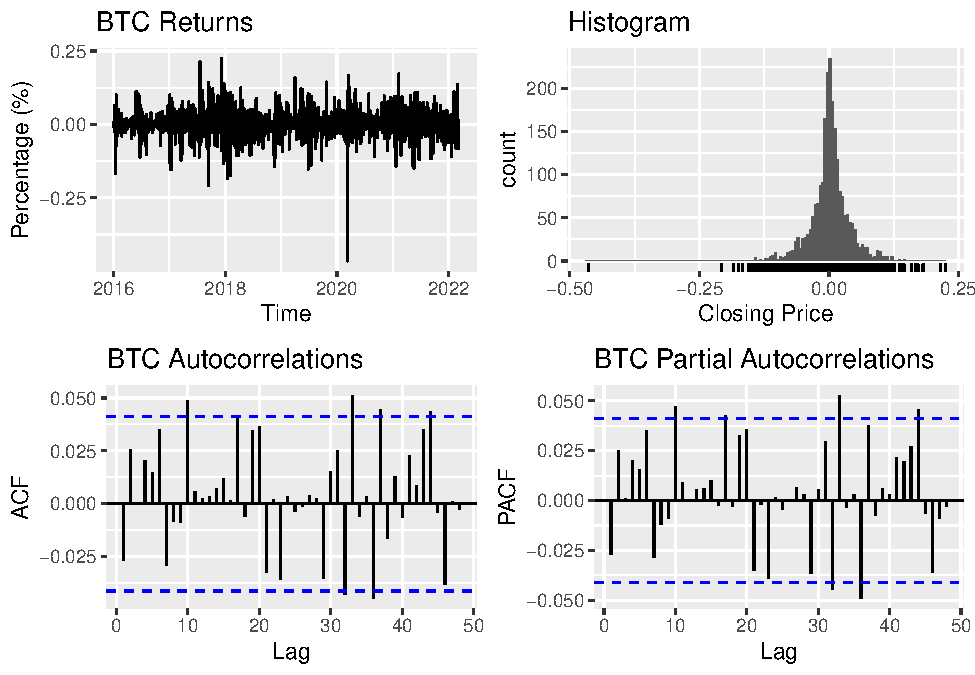
\includegraphics{project2_files/figure-latex/unnamed-chunk-3-1.pdf}

\begin{Shaded}
\begin{Highlighting}[]
\FunctionTok{autoplot}\NormalTok{(}\FunctionTok{stl}\NormalTok{(tup\_ts,}\AttributeTok{s.window =} \StringTok{"periodic"}\NormalTok{,}\AttributeTok{robust=}\ConstantTok{TRUE}\NormalTok{),}
     \AttributeTok{main =} \StringTok{"TUP STL Decomposition"}\NormalTok{)}
\end{Highlighting}
\end{Shaded}

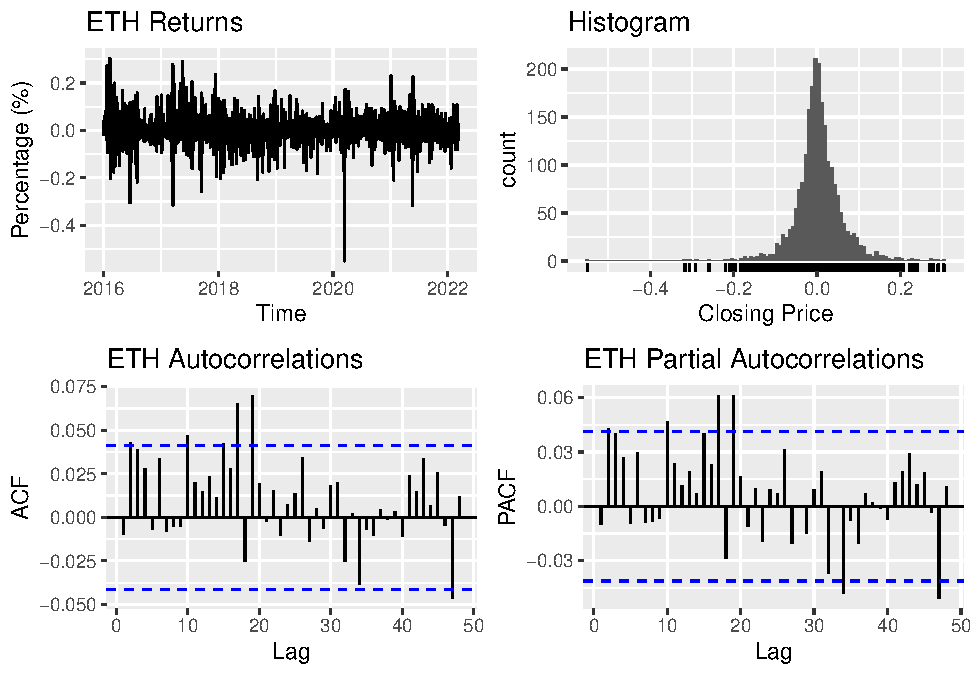
\includegraphics{project2_files/figure-latex/unnamed-chunk-3-2.pdf}

\begin{Shaded}
\begin{Highlighting}[]
\FunctionTok{autoplot}\NormalTok{(}\FunctionTok{stl}\NormalTok{(sp500\_ts,}\AttributeTok{s.window =} \StringTok{"periodic"}\NormalTok{,}\AttributeTok{robust=}\ConstantTok{TRUE}\NormalTok{),}
     \AttributeTok{main =} \StringTok{"S\&P 500 STL Decomposition"}\NormalTok{)}
\end{Highlighting}
\end{Shaded}

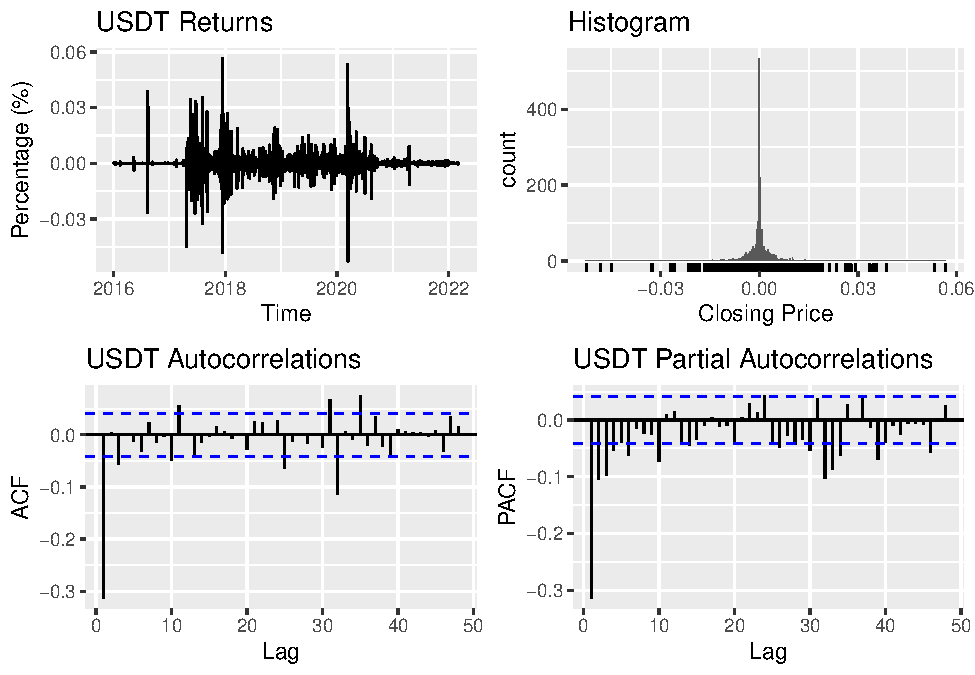
\includegraphics{project2_files/figure-latex/unnamed-chunk-3-3.pdf}

Each decomposition shows that the the time series have significant
trend, seasonality, and cycle components. Morever, it shows that each
series is not covariance stationary, which we will need to consider when
producing models.

SNBR's price trend is mostly upward with some drift at the end of the
observed time period. The seasonality of the data looks quite consistent
over time, and there are significant cycles in the data, particularly in
the last 4 years of the time series.

TUP's price follows a downward trend with some drift. Generally, it
fluctuates more than the trend of SNBR's price. The seasonality of the
data exhibits more persistence than SNBR's, and it looks consistent over
time. The cycles in TUP's price data are very clear and much more
significant than what can be observed in SNBR's remainders.

S\&P 500's price trend is quite linear and upward sloping. The
seasonality of the data looks persistent and consistent over time, and
there is significant evidence of cycles in the residuals data,
particularly in the last 4 years of the time series.

\hypertarget{c-e-fit-a-model-that-includes-trend-seasonality-and-cyclical-components.-then-plot-the-acf-and-pacf-of-the-respective-residuals-and-interpret-the-plots.}{%
\subsection{(C) \& (E): Fit a model that includes, trend, seasonality,
and cyclical components. Then plot the ACF and PACF of the respective
residuals and interpret the
plots.}\label{c-e-fit-a-model-that-includes-trend-seasonality-and-cyclical-components.-then-plot-the-acf-and-pacf-of-the-respective-residuals-and-interpret-the-plots.}}

To capture the complex dynamics of the series, we will be fitting an
ARIMA model to each of them.

\hypertarget{snbr-price}{%
\subsubsection{SNBR Price}\label{snbr-price}}

\begin{Shaded}
\begin{Highlighting}[]
\NormalTok{m1 }\OtherTok{\textless{}{-}} \FunctionTok{auto.arima}\NormalTok{(snbr\_ts)}
\FunctionTok{summary}\NormalTok{(m1)}
\end{Highlighting}
\end{Shaded}

\begin{verbatim}
## Series: snbr_ts 
## ARIMA(2,1,0)(0,0,1)[52] 
## 
## Coefficients:
##           ar1     ar2     sma1
##       -0.0811  0.1941  -0.1251
## s.e.   0.0407  0.0412   0.0499
## 
## sigma^2 = 7.981:  log likelihood = -1426.75
## AIC=2861.5   AICc=2861.57   BIC=2878.96
## 
## Training set error measures:
##                     ME     RMSE      MAE       MPE     MAPE      MASE
## Training set 0.1175282 2.815382 1.730309 0.1159322 4.886237 0.1310172
##                      ACF1
## Training set -0.004760446
\end{verbatim}

The model for the price of SNBR is ARIMA (2,1,0) + weekly
Seasonal-ARIMA(0,0,2). The I = 1 affirms that the data is not covariance
stationary, which is important when modelling with short-term memory
processes such as AR and MA processes.

The seasonality of the data is captured by the seasonal component of the
model. Specifically, it is taken care of by an S-MA(1). The trend of the
series is taken care of by the first differencing I(1), and the cycles
of the data are modelled by an AR(2) process.

\begin{Shaded}
\begin{Highlighting}[]
\FunctionTok{ggtsdisplay}\NormalTok{(}\FunctionTok{resid}\NormalTok{(m1))}
\end{Highlighting}
\end{Shaded}

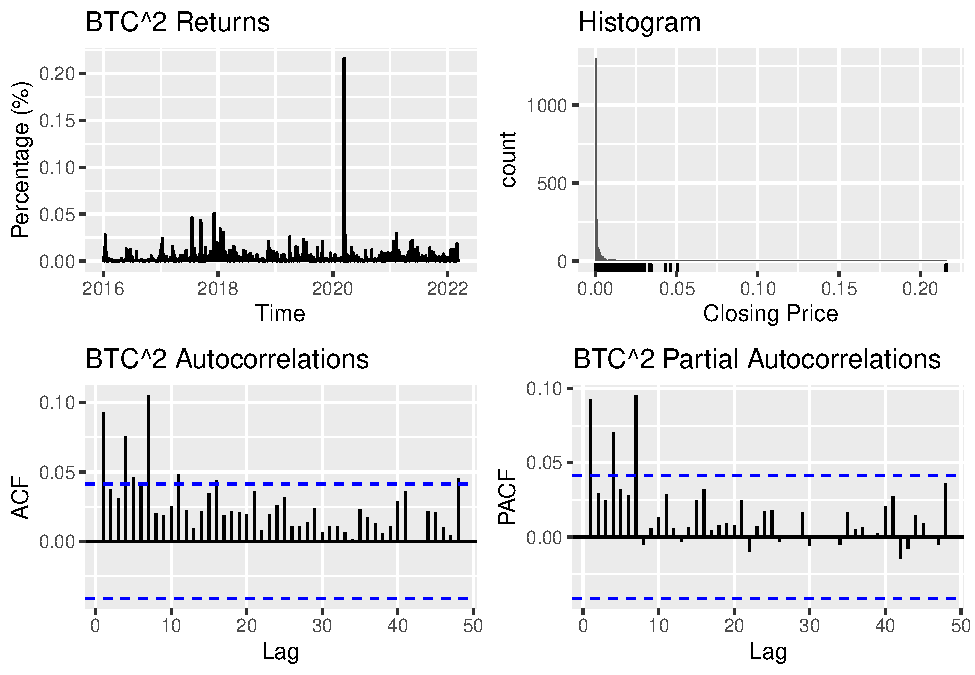
\includegraphics{project2_files/figure-latex/unnamed-chunk-4-1.pdf}

The plot of the residuals appears to retain some structure which can be
modelled. However, the magnitude of the autocorrelation spikes seen on
the ACF and PACF plots suggest that this structure may not be very
significant. Therefore, the ARIMA(2,1,0) + S-ARIMA(0,0,1) model fits the
data quite well.

\hypertarget{tup-price}{%
\subsubsection{TUP Price}\label{tup-price}}

\begin{Shaded}
\begin{Highlighting}[]
\NormalTok{m2 }\OtherTok{\textless{}{-}} \FunctionTok{auto.arima}\NormalTok{(tup\_ts)}
\FunctionTok{summary}\NormalTok{(m2)}
\end{Highlighting}
\end{Shaded}

\begin{verbatim}
## Series: tup_ts 
## ARIMA(1,1,2)(1,0,0)[52] 
## 
## Coefficients:
##           ar1     ma1     ma2     sar1
##       -0.7589  0.7348  0.0540  -0.0011
## s.e.   0.1448  0.1484  0.0462   0.0445
## 
## sigma^2 = 5.321:  log likelihood = -1308.02
## AIC=2626.04   AICc=2626.15   BIC=2647.87
## 
## Training set error measures:
##                       ME     RMSE      MAE        MPE    MAPE      MASE
## Training set -0.05496745 2.296764 1.601122 -0.5604413 4.68789 0.1035682
##                      ACF1
## Training set -0.001781102
\end{verbatim}

The model for the price of TUP is ARIMA (1,1,2) + weekly
Seasonal-ARIMA(1,0,0). The I = 1 affirms that the data is not covariance
stationary, which is important when modelling with short-term memory
processes such as AR and MA processes.

The seasonality of the data is captured by the seasonal component of the
model. Specifically, it is taken care of by an S-AR(1) process. The
trend of the series is taken care of by the first differencing I(1), and
the cycles of the data are modelled by an ARMA(1,2) process.

\begin{Shaded}
\begin{Highlighting}[]
\FunctionTok{ggtsdisplay}\NormalTok{(}\FunctionTok{resid}\NormalTok{(m2))}
\end{Highlighting}
\end{Shaded}

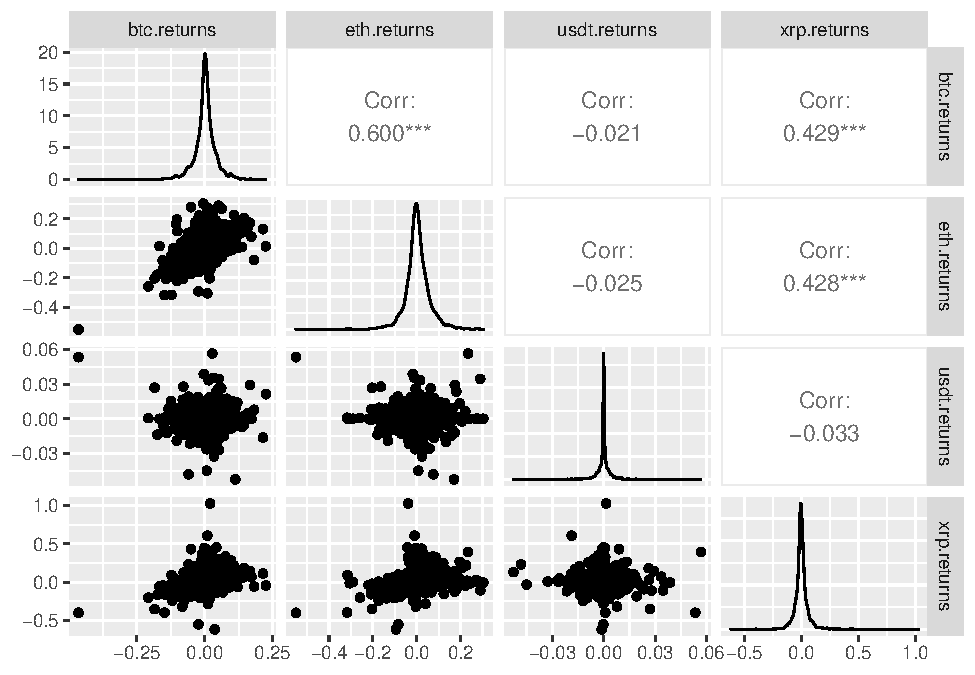
\includegraphics{project2_files/figure-latex/unnamed-chunk-5-1.pdf}

The plot of the residuals appears to have no structure. This intuition
is affirmed by the ACF and PACF plots which do not have significant
spikes. Thus, the ARIMA (1,1,2) + S-ARIMA(1,0,0) model fits the data
very well.

\hypertarget{sp-500-price}{%
\subsubsection{S\&P 500 Price}\label{sp-500-price}}

\begin{Shaded}
\begin{Highlighting}[]
\NormalTok{m3 }\OtherTok{\textless{}{-}} \FunctionTok{auto.arima}\NormalTok{(sp500\_ts)}
\FunctionTok{summary}\NormalTok{(m3)}
\end{Highlighting}
\end{Shaded}

\begin{verbatim}
## Series: sp500_ts 
## ARIMA(0,1,1) with drift 
## 
## Coefficients:
##           ma1   drift
##       -0.0829  5.5559
## s.e.   0.0400  2.1442
## 
## sigma^2 = 3186:  log likelihood = -3166.73
## AIC=6339.47   AICc=6339.51   BIC=6352.56
## 
## Training set error measures:
##                       ME     RMSE      MAE         MPE     MAPE      MASE
## Training set 0.003129593 56.29953 35.83029 -0.07692124 1.508007 0.1105106
##                      ACF1
## Training set -0.003033807
\end{verbatim}

The model for the price of the S\&P 500 is ARIMA(0,1,1) + drift. The
drift suggests that there is a non-intercept for our model's fit. The I
= 1 affirms that the data is not covariance stationary, which is
important when modelling with short-term memory processes such as AR and
MA processes.

There is no seasonal component in this model, suggesting that the
seasonality is correctly captured by the ARIMA(0,1,1) model. The trend
of the series is taken care of by the first differencing I(1), and the
cycles of the data are modelled by an MA(1) process.

\begin{Shaded}
\begin{Highlighting}[]
\FunctionTok{ggtsdisplay}\NormalTok{(}\FunctionTok{resid}\NormalTok{(m3))}
\end{Highlighting}
\end{Shaded}

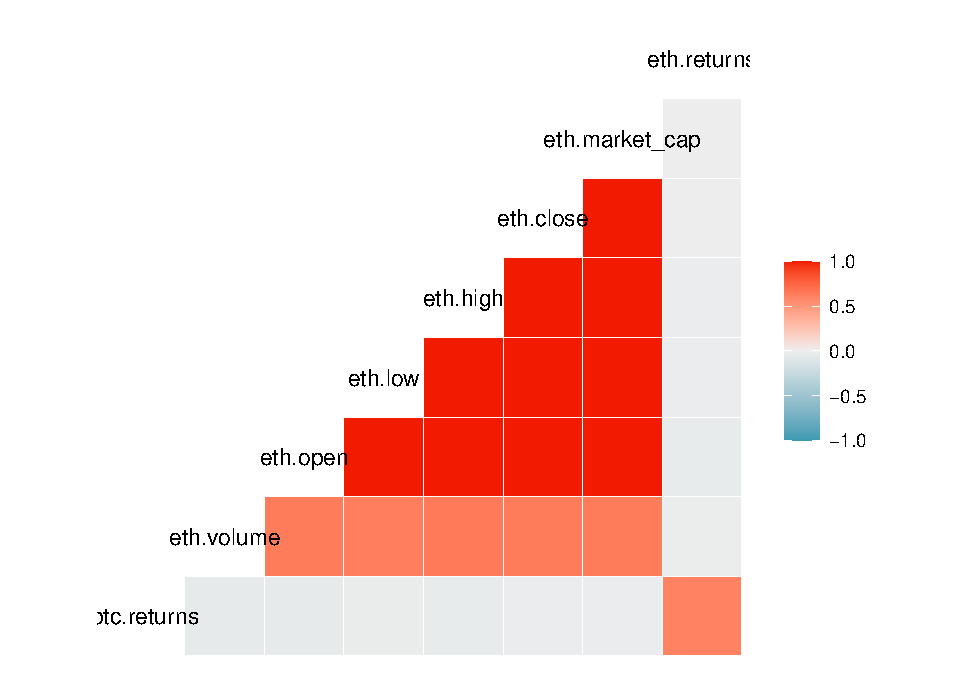
\includegraphics{project2_files/figure-latex/unnamed-chunk-7-1.pdf}

The plot of the residuals appears to retain some structure which can be
modelled. The residuals are also heteroskedastic. However, the magnitude
of the autocorrelation spikes seen on the ACF and PACF plots suggest
that this structure may not be very significant. Therefore, the
ARIMA(0,1,1) + drift model fits the data quite well.

\hypertarget{d-plot-the-respective-residuals-vs.-fitted-values-and-discuss-your-observations.}{%
\subsection{(D) Plot the respective residuals vs.~fitted values and
discuss your
observations.}\label{d-plot-the-respective-residuals-vs.-fitted-values-and-discuss-your-observations.}}

\hypertarget{snbr-model-residuals-vs-fit}{%
\subsubsection{SNBR Model Residuals vs
Fit}\label{snbr-model-residuals-vs-fit}}

\begin{Shaded}
\begin{Highlighting}[]
\NormalTok{plot\_resid\_fit }\OtherTok{\textless{}{-}} \ControlFlowTok{function}\NormalTok{(x,y) \{}
\NormalTok{  data }\OtherTok{=} \FunctionTok{data.frame}\NormalTok{(}\AttributeTok{x =}\NormalTok{ x, }\AttributeTok{y =}\NormalTok{ y)}

\NormalTok{  p }\OtherTok{\textless{}{-}} \FunctionTok{ggplot}\NormalTok{(data, }\FunctionTok{aes}\NormalTok{(}\AttributeTok{x =}\NormalTok{  x, }\AttributeTok{y =}\NormalTok{ y)) }\SpecialCharTok{+}
    \FunctionTok{geom\_smooth}\NormalTok{(}\AttributeTok{method =} \StringTok{"lm"}\NormalTok{, }\AttributeTok{se=}\NormalTok{T,}
                \AttributeTok{col =} \StringTok{"red"}\NormalTok{,}
                \AttributeTok{formula =}\NormalTok{ y }\SpecialCharTok{\textasciitilde{}}\NormalTok{ x,}
                \AttributeTok{show.legend =}\NormalTok{ T) }\SpecialCharTok{+} 
    \FunctionTok{geom\_point}\NormalTok{(}\AttributeTok{alpha =} \FloatTok{0.5}\NormalTok{,}\AttributeTok{size =} \DecValTok{2}\NormalTok{,}
               \AttributeTok{col =} \StringTok{"black"}\NormalTok{) }\SpecialCharTok{+}
    \FunctionTok{xlab}\NormalTok{(}\StringTok{"Fit"}\NormalTok{) }\SpecialCharTok{+} \FunctionTok{ylab}\NormalTok{(}\StringTok{"Residuals"}\NormalTok{) }\SpecialCharTok{+}
    \FunctionTok{ggtitle}\NormalTok{(}\StringTok{"Residuals vs Fit"}\NormalTok{) }
    
  \FunctionTok{return}\NormalTok{(p)}
\NormalTok{\}}

\FunctionTok{plot\_resid\_fit}\NormalTok{(}\FunctionTok{fitted}\NormalTok{(m1),}\FunctionTok{resid}\NormalTok{(m1))}
\end{Highlighting}
\end{Shaded}

\begin{verbatim}
## Don't know how to automatically pick scale for object of type ts. Defaulting to continuous.
## Don't know how to automatically pick scale for object of type ts. Defaulting to continuous.
\end{verbatim}

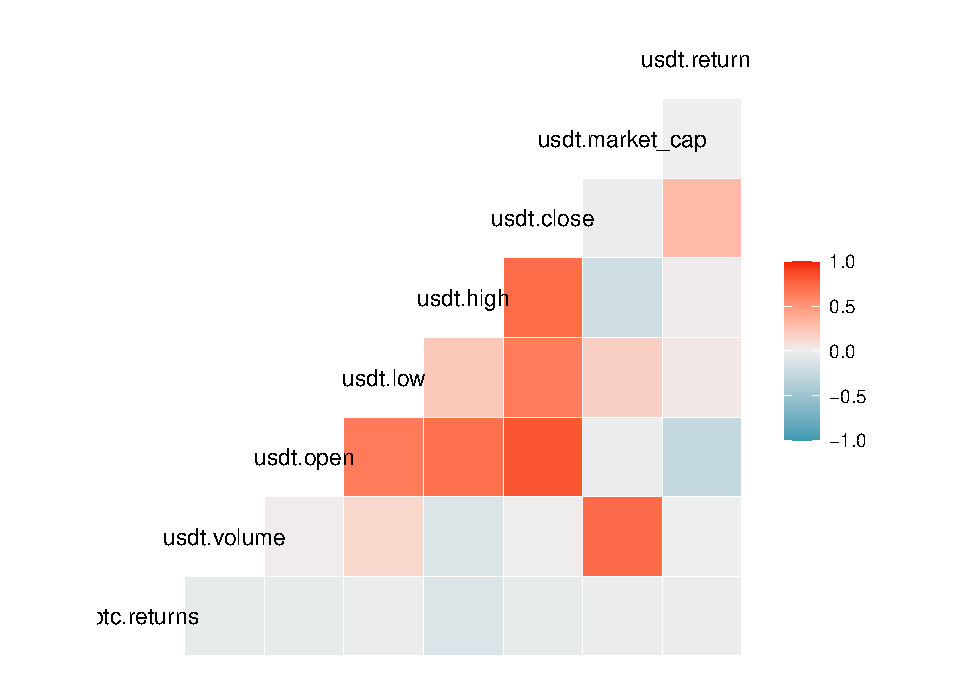
\includegraphics{project2_files/figure-latex/unnamed-chunk-8-1.pdf}

There is not much of a linear relationship between the fit and the
residuals, suggesting affirming that our model's fit did pretty well.

\hypertarget{tup-model-residuals-vs-fit}{%
\subsubsection{TUP Model Residuals vs
Fit}\label{tup-model-residuals-vs-fit}}

\begin{Shaded}
\begin{Highlighting}[]
\FunctionTok{plot\_resid\_fit}\NormalTok{(}\FunctionTok{fitted}\NormalTok{(m2),}\FunctionTok{resid}\NormalTok{(m2))}
\end{Highlighting}
\end{Shaded}

\begin{verbatim}
## Don't know how to automatically pick scale for object of type ts. Defaulting to continuous.
## Don't know how to automatically pick scale for object of type ts. Defaulting to continuous.
\end{verbatim}

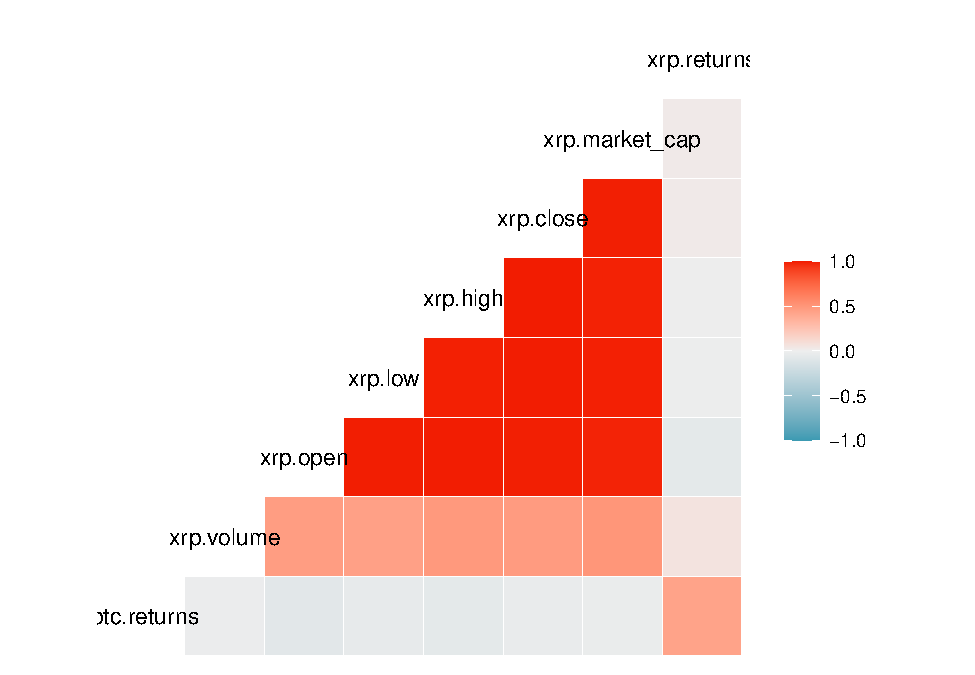
\includegraphics{project2_files/figure-latex/unnamed-chunk-9-1.pdf}

There is basically no linear relationship between the residuals and the
fitted data. Therefore, our model for TUP prices did exceptionally well.

\hypertarget{sp-500-model-residuals-vs-fit}{%
\subsubsection{S\&P 500 Model Residuals vs
Fit}\label{sp-500-model-residuals-vs-fit}}

\begin{Shaded}
\begin{Highlighting}[]
\FunctionTok{plot\_resid\_fit}\NormalTok{(}\FunctionTok{fitted}\NormalTok{(m3),}\FunctionTok{resid}\NormalTok{(m3))}
\end{Highlighting}
\end{Shaded}

\begin{verbatim}
## Don't know how to automatically pick scale for object of type ts. Defaulting to continuous.
## Don't know how to automatically pick scale for object of type ts. Defaulting to continuous.
\end{verbatim}

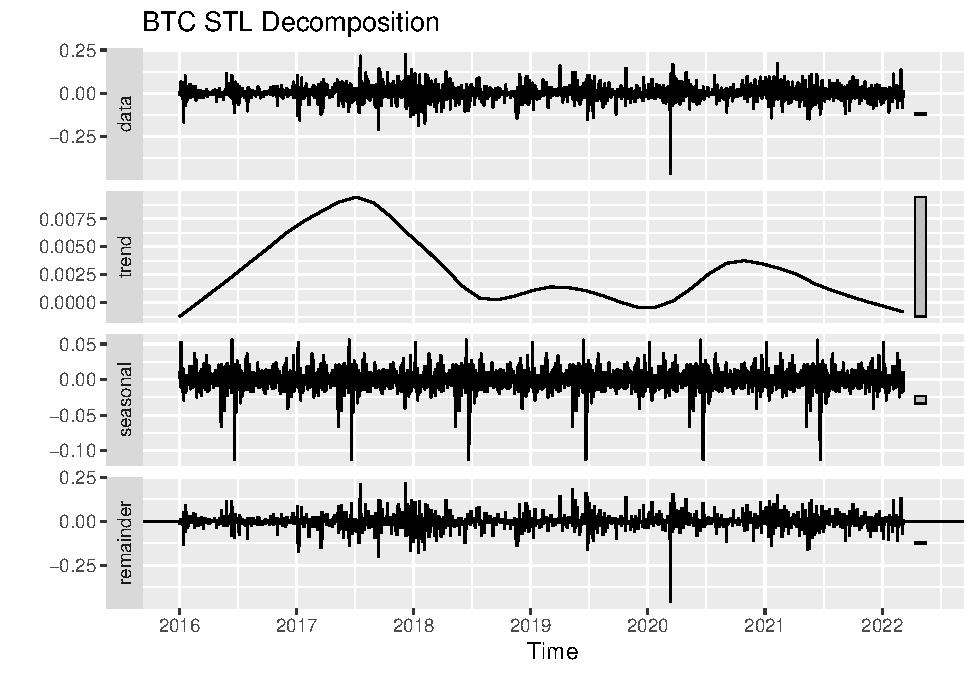
\includegraphics{project2_files/figure-latex/unnamed-chunk-10-1.pdf}

There is also, no linear relationship between the residuals and the fit
of the model fitted to the S\&P 500 price series. Therefore, our ARIMA
model for this data did very well in fitting the series

\hypertarget{f-plot-the-respective-cusum-and-interpret-the-plot.}{%
\subsection{(F) Plot the respective CUSUM and interpret the
plot.}\label{f-plot-the-respective-cusum-and-interpret-the-plot.}}

\hypertarget{g-for-your-model-discuss-the-associated-diagnostic-statistics.}{%
\subsection{(G) For your model, discuss the associated diagnostic
statistics.}\label{g-for-your-model-discuss-the-associated-diagnostic-statistics.}}

\hypertarget{h-use-your-model-to-forecast-12-steps-ahead.-your-forecast-should-include-the-respective-error-bands.}{%
\subsection{(H) Use your model to forecast 12-steps ahead. Your forecast
should include the respective error
bands.}\label{h-use-your-model-to-forecast-12-steps-ahead.-your-forecast-should-include-the-respective-error-bands.}}

\hypertarget{i-compare-your-forecast-from-i-to-the-12-steps-ahead-forecasts-from-arima-holt-winters-and-ets-models.-which-model-performs-best-in-terms-of-mape}{%
\subsection{(I) Compare your forecast from (i) to the 12-steps ahead
forecasts from ARIMA, Holt-Winters, and ETS models. Which model performs
best in terms of
MAPE?}\label{i-compare-your-forecast-from-i-to-the-12-steps-ahead-forecasts-from-arima-holt-winters-and-ets-models.-which-model-performs-best-in-terms-of-mape}}

\hypertarget{j-combine-the-four-forecasts-and-comment-on-the-mape-from-this-forecasts-vs.-the-individual-ones.}{%
\subsection{(J) Combine the four forecasts and comment on the MAPE from
this forecasts vs., the individual
ones.}\label{j-combine-the-four-forecasts-and-comment-on-the-mape-from-this-forecasts-vs.-the-individual-ones.}}

PHAM STOPS HERE

\hypertarget{k-fit-an-appropriate-var-model-using-your-two-variables.-make-sure-to-show-the-relevant-plots-and-discuss-your-results-from-the-fit.}{%
\subsection{(K) Fit an appropriate VAR model using your two variables.
Make sure to show the relevant plots and discuss your results from the
fit.}\label{k-fit-an-appropriate-var-model-using-your-two-variables.-make-sure-to-show-the-relevant-plots-and-discuss-your-results-from-the-fit.}}

\hypertarget{l-compute-plot-and-interpret-the-respective-impulse-response-functions.}{%
\subsection{(L) Compute, plot, and interpret the respective impulse
response
functions.}\label{l-compute-plot-and-interpret-the-respective-impulse-response-functions.}}

\hypertarget{m-perform-a-granger-causality-test-on-your-variables-and-discuss-your-results-from-the-test.}{%
\subsection{(M) Perform a Granger-Causality test on your variables and
discuss your results from the
test.}\label{m-perform-a-granger-causality-test-on-your-variables-and-discuss-your-results-from-the-test.}}

\hypertarget{n-use-your-var-model-to-forecast-12-steps-ahead.-your-forecast-should-include-the-respective-error-bands.-comment-on-the-differences-between-the-var-forecast-and-the-other-ones-obtained-using-the-different-methods.}{%
\subsection{(N) Use your VAR model to forecast 12-steps ahead. Your
forecast should include the respective error bands. Comment on the
differences between the VAR forecast and the other ones obtained using
the different
methods.}\label{n-use-your-var-model-to-forecast-12-steps-ahead.-your-forecast-should-include-the-respective-error-bands.-comment-on-the-differences-between-the-var-forecast-and-the-other-ones-obtained-using-the-different-methods.}}

\newpage

\hypertarget{iii.-conclusions-and-future-work}{%
\section{III. Conclusions and Future
Work}\label{iii.-conclusions-and-future-work}}

\newpage

\hypertarget{iv.-references}{%
\section{IV. References}\label{iv.-references}}

\newpage

\hypertarget{v.-r-source-code}{%
\section{V. R Source Code}\label{v.-r-source-code}}

\end{document}
